% Dokumentace projektu IFJ a IAL
% Vytvořil: Lukáš Šidlík ; xsidlil00 

\documentclass[a4paper, 11pt]{article}

\usepackage[czech]{babel}
\usepackage[utf8]{inputenc}
\usepackage[T1]{fontenc}
\usepackage[left=2cm, text={17cm, 25cm}, top=2cm, a4paper]{geometry}
\usepackage{hyperref}
\usepackage{graphicx}
\usepackage{tabularx,booktabs}
\usepackage{array}
\usepackage{makecell} 
\usepackage{pdflscape}
\usepackage{amsmath,bm}
\usepackage{listings}
\usepackage{wrapfig}
\usepackage[export]{adjustbox}

\newcolumntype{Y}{>{\centering\arraybackslash}X}
\newcolumntype{?}{!{\vrule width 0.15em}}

\begin{document}

\begin{titlepage}
    \begin{center}
        \Huge{\textsc{Vysoké učení technické v Brně}} \\
        \huge{\textsc{Fakulta informačních technologií}} \\
        \vspace{\stretch{0.191}}
        \begin{figure}[h]
            \centering
            \scalebox{0.14}{\includegraphics{pictures/FIT_barevne_RGB_CZ.png}} 
        \end{figure}
        \vspace{\stretch{0.128}}
        \LARGE{Dokumentace k projektu do předmětu IFJ a IAL} \\[0,05em]
        \Huge{Implementace překladače jazyka IFJ24}\\[0,2em]
        \Large{Tým xhubacv00, varianta - TRP-izp}
        \vspace{\stretch{0.618}}
    \end{center}

    \hfill
    \begin{minipage}{\textwidth}
        \large
        \begin{tabbing}
            Vodní melouny sleva \= cukr káva limonáda r  \= před pikolou  \= rum bum \kill
            \textbf{Vedoucí týmu:} \> Vojtěch Hubáček \> xhubacv00 \> 25\% \\
            \textbf{Členové týmu:}  \> Jakub Ramašeuski \> xramas01 \> 25\% \\
            \> Jozef Ondrejička \> xondre16 \> 25\% \\
            \> Lukáš Šidlík \> xsidlil00 \> 25\% \\
        \end{tabbing} 
    \end{minipage}
        
    \begin{minipage}{0.5 \textwidth}
        \large
        \today
    \end{minipage}
\end{titlepage}

%%%%%%%%%%%%%%%%%%%%%%%%%%%%%%%%%%%%%%%%%%%%%%%%%%%%%%%%%%%%%%%%%%%%%%%%%%%%%%%%%%%%%%%%%%%%%%%%%%%%%
% Obsah
\begin{titlepage}
    \tableofcontents
\end{titlepage}
\setcounter{page}{1}

%%%%%%%%%%%%%%%%%%%%%%%%%%%%%%%%%%%%%%%%%%%%%%%%%%%%%%%%%%%%%%%%%%%%%%%%%%%%%%%%%%%%%%%%%%%%%%%%%%%%%
% Úvod

\section{Úvod}

Cílem projektu bylo vytvořit překladač, který načte cílový kód jazyka IFJ24, který je podmnožinou programovacího jazyka Zig a přeloží ho do cílového jazyka IFJcode24. 

V případě úspěchu překladu se na standardní výstup vypíše cílový kód jazyku IFJcode24, jinak program skončí s daným číslem chyby a chybovou hláškou.

%%%%%%%%%%%%%%%%%%%%%%%%%%%%%%%%%%%%%%%%%%%%%%%%%%%%%%%%%%%%%%%%%%%%%%%%%%%%%%%%%%%%%%%%%%%%%%%%%%%%%
% Implementace překladače
\section{Implementace překladače IFJ24} 

V této kapitole jsou rozepsané dílčí části programu a komunikace mezi nimi.

%%%%%%%%%%%%%%%%%%%%%%%%%%%%%%%%%%%%%%%%%%%%%%%%%%%%%%%%%%%%%%%%%%%%%%%%%%%%%%%%%%%%%%%%%%%%%%%%%%%%%
% Lexikální analýza
\subsection{Lexikální analýza}

Skener se snaží co nejvíc přiblížit návrhu, je tedy zaveden jako orientovaný graf pod jmennými prostory \verb|scn (SCaNner)| a \verb|sca (SCanner Auxiliary)|, z nichž \verb|scn| je využit zejména pro komunikaci skeneru ven a sca pro jeho konfiguraci. 

V kódu \verb|sca| tím vzniklo rozhraní pro konfiguraci orientovaného grafu, které dovoluje deklaraci hran s pomocí \verb|SCA_PATH_DECL(src, dest)|, definici s \verb|SCA_PATH_DEF(src, dest)| inicializaci s \verb|SCA_PATH_INIT| \verb|(name, args...)|, kterýmž lze dosadit hraně se jménem name dosadit disjunktní podmínky \verb|(args)|, tedy stačí, aby z N podmínek platila jedna pro zvolení dané cesty, zmínění hrany 
\verb|SCA_PATH(src, dest)| a deiniciaci orientovaných hran mezi uzly, které jsou sice deklarovány globálně, nicméně jim jsou hrany dosazeny až v rámci běhu programu za pomocí funkce \verb|sca_assign_children(Scan_node_ptr node, |\\ \verb|int argc, ...)| s variabilním počtem argumentů.

Celý běh skeneru tím lze soustředit do funkce \verb|scn_scan|, jenž iterativně prochází řetězec pomocí deterministického konečného automatu viz(\ref{DKA}), dokud nenarazí na situaci, kdy pro načtený symbol nevede z daného uzlu přechod.
Tehdy je načtený řetězec nejdříve vyhodnocen dle toho, zda se automat zastavil na terminálu definovaném v tabulce \verb|sca_translation_table[]|, pokud ano, na jakém a vyhodí příslušný \verb|token|, v opačném případě skener vyhodí chybu a ukončí program.
V případě setkání se se symbolem konce řetězce \verb|EOF| zastavuje načítání řetězce a v případě požadavku na další token jej pro usnadnění práce načte z dvousměrně vázaného seznamu.

\subsubsection{Příklad užití rozhraní lexikální analýzy}
\begin{wrapfigure}{r}{0.3\textwidth}
\scalebox{0.95}{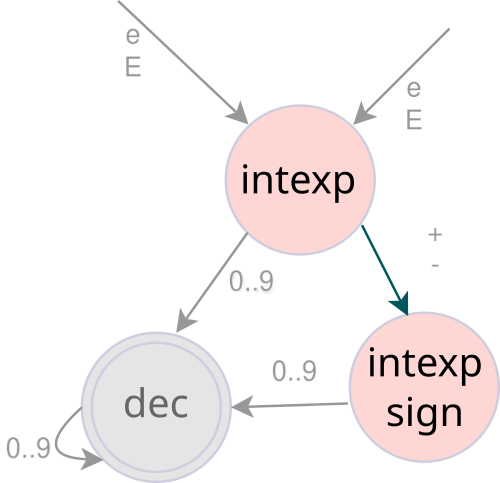
\includegraphics{pictures/scanner_dfa_example.png}}
\raggedright
\caption{uváděné uzly a hrany (barevně)}
\end{wrapfigure}
Zde jsou uvedeny příklady užití. Pro tento příklad uvažujme existenci hrany mezi uzlem, který v číslu představuje exponent (\verb|sca_intexp|) a znaménko (\verb|sca_intexpsign|). Průchod přes hranu je tedy dovolen pouze pokud je načtený symbol plus nebo minus.
\begin{itemize}
    \item \verb|SCA_PATH_DEF(sca_intexp, sca_intexpsign)|
    \begin{itemize}
        \item tímto je definována hrana mezi uzlem \verb|sca_intexp| a \verb|sca_intexpsign|
    \end{itemize}
    \item \verb|SCA_PATH_INIT(SCA_PATH(sca_intexp, sca_intexpsign),|\\ \verb|SCA_MATCH(plus), SCA_MATCH(minus))|
    \begin{itemize}
        \item tímto jsou za běhu hraně dosazeny podmínky požadující znaménka plus nebo minus
    \end{itemize}
    \item \verb|sca_assign_children(&sca_intexp, 2, &SCA_PATH|\\ \verb|(sca_intexp, sca_dec2), &SCA_PATH(sca_intexp, sca_intexpsign));|
    \begin{itemize}
        \item tímto jsou uzlu dosazeny hrany, které z něj vedou. Z uzlu tímto lze přejít do jiného s jiným stavem, zároveň je uzel zodpovědný za následnou deiniciaci hran při ukončení programu. V našem případu to znamená, že z uzlu vedou hrany do uzlů \verb|sca_intexpsign| a terminálního \verb|sca_dec2|
    \end{itemize}
\end{itemize}

%%%%%%%%%%%%%%%%%%%%%%%%%%%%%%%%%%%%%%%%%%%%%%%%%%%%%%%%%%%%%%%%%%%%%%%%%%%%%%%%%%%%%%%%%%%%%%%%%%%%%
% Syntaktická analýza
\subsection{Syntaktická analýza}

Syntaktická analýza v tomto projektu je implementována jako dvoufázový proces, který zajišťuje správné zpracování zdrojového kódu a přípravu na generování výsledného kódu. 
Naše syntaktická analýza byla implementována pomocí metody rekurzivního sestupu založeného na LL\--gramatice (vše kromě výrazů), viz (\ref{GRA}), což umožňuje přehledné a systematické zpracování jednotlivých syntaktických konstrukcí.

První fáze, realizovaná funkcí \verb|parse_fn_first|, provádí základní syntaktickou kontrolu zdrojového kódu, identifikuje deklarace funkcí, jejich parametry a ukládá je do tabulky symbolů. 
Druhá fáze, která začíná inicializací zásobníku a řetězců pro generování kódu, spouští syntaktickou analýzu z neterminálu \verb|<program>| pomocí funkce program a postupně zpracovává jednotlivé části programu, jako jsou deklarace, parametry, tělo funkcí a příkazy.

Syntaktická analýza zahrnuje hlavně práci s neterminály, jako například \verb|<prolog>|, \verb|<function>|, \verb|<body>|, \verb|<statement>| či \verb|<call>|.
Tento dvoufázový přístup zaručuje efektivní sémantickou kontrolu a generování správného výstupního kódu, což tvoří základ pro další zpracování výrazů, ve kterých se volají funkce a generování tříadresného kódu.
%%%%%%%%%%%%%%%%%%%%%%%%%%%%%%%%%%%%%%%%%%%%%%%%%%%%%%%%%%%%%%%%%%%%%%%%%%%%%%%%%%%%%%%%%%%%%%%%%%%%%
% Zpracování výrazů
\subsubsection{Zpracování výrazů}

Syntaktická analýza výrazu je v souboru \verb|parser.c| řízena precedenční analýzou, k níž je vytvořena odpovídající precedenční tabulka. 
Syntaktická analýza přistupuje v podstatě ke všemu jako k výrazu, přestože se může skládat například jen z jednoho literálu.  
Precedenční analýza je řízena operacemi posuvu \verb|'<'|, pouhého vložení \verb|'='|, prázdné operace \verb|' '| a redukce \verb|'>'| s použitím odpovídajících pravidel (\verb|E| $\rightarrow$ \verb|ID|, \verb|E| $\rightarrow$ \verb|(E)| ,\verb|E| $\rightarrow$ \verb|!E|, \verb|E| $\rightarrow$ \verb|E.?|, \verb|E| $\rightarrow$ \verb|E|$\{+|-|*|/|orelse|==|!=|<|>|<=|>=|and|or\}$\verb|E|).
Současně s precedenční analýzou je vytvářena postfixová notace výrazu pro kontrolu sémantickou analýzou a pro následnou generaci cílového kódu.

%%%%%%%%%%%%%%%%%%%%%%%%%%%%%%%%%%%%%%%%%%%%%%%%%%%%%%%%%%%%%%%%%%%%%%%%%%%%%%%%%%%%%%%%%%%%%%%%%%%%%
% Sémantická analýza
\subsection{Sémantická analýza}

Se syntaktickou analýzou je v \verb|parser.c| zároveň implementována analýza sémantická.
Ve struktuře \verb|parser_tools_t|, která je definována v \verb|parser.h| jsou uloženy všechny struktury a proměnné, které jsou nezbytné pro sémantickou kontrolu.

Při prvním průchodu se naplní symbolická tabulka viz(\ref{TRP}) funkcí, jelikož v jazyce IFJ24 nezáleží jestli je volaná funkce definována nad nebo pod jejím voláním. 
V tomhle průchodu se zkontroluje i redefinice funkcí.

Při druhém průchodu už se provádí všechny zbylé sémantické kontroly v tělech funkcí, a plnění symbolický tabulek proměnných, které jsou uloženy v dvousměrně vázaném seznamu (ten je implementovaný \verb|symDLList.c|), který se nachází v \verb|perser_tools_t|. 
U každého paměťovém bloku (\verb|if, while, else|) se vytvoří nová symbolická tabulka a vloží se na konec obousměrně vázaného seznamu. 
Po odejití z bloku se zkontroluje použití všech proměnných, které byly v daném bloku definovány a následně se tabulka zničí.
Na konci sémantické analýzy se zkontroluje jestli existuje funkce \verb|main|.

Kontrola datové kompatibility ve výrazech se řeší v \verb|expression.c|, kde se odvodí datový typ výsledku a zkontrolují validní implicitní konverze. 
Dále se podle kontextu zkontroluje, jestli daný výsledek má správný datový typ, vůči čemu byl volán \verb|(if, return)| nebo přiřazení.

%%%%%%%%%%%%%%%%%%%%%%%%%%%%%%%%%%%%%%%%%%%%%%%%%%%%%%%%%%%%%%%%%%%%%%%%%%%%%%%%%%%%%%%%%%%%%%%%%%%%%
% Generování cílového kódu
\subsection{Generování cílového kódu}

Generace kódu probíhá přímo v souboru \verb|parser.c| při druhém průchodu parseru zdrojovým kódem. 
Všechny potřebné funkce, formáty instrukcí a další pomocné konstrukce pro generování cílového kódu jsou umístěny  v souboru \verb|codegen.c| a \verb|codegen.h|.

\subsubsection{Generace instrukcí}

Pro instrukce bylo v souboru \verb|codegen.c| předpřipraveno pole formátu instrukcí cílového jazyka pro bezpečnější práci s instrukcemi  \cite{el-husa}. 
Vytvoření jednoznačných proměnných a návěští je řešeno pomocí počítadel dostupných v nástrojích parseru určených pro generátor kódu.

\subsubsection{Průběžná generace celkového kódu}

K výpisu jednotlivých instrukcí zdrojového kódu se souboru \verb|parser.c| využívá předpřipravené makro \verb|printi|. 
Toto makro přijímá formátovaný řetězec s již danou instrukcí a argumenty pro formátovaný řetězec, jimiž jsou hodnoty užívané instrukcí. 
Cílový kód programu je následně makrem vypisován v závislosti na typu instrukce do dynamických řetězců typu \verb|str_t| nacházejících se v nástrojích parseru. 

Tedy takřka všechny instrukce jsou zapisovány do dočasného řetězce, až na instrukci definice proměnné \verb|DEFVAR|, která je přednostně zapisována do hlavního řetězce instrukcí za vstupem do dané funkce (jelikož definice proměnných nelze pro provádět uvnitř cyklů, kvůli redefinici proměnných). 
Na konci každé funkce je hlavní a dočasný řetězec sjednocen. 

Vestavěné funkce a pomocné funkce zpracování výrazů jsou generovány na konci průchodu parseru zdrojovým programem. 
Na závěr v případě, že je zdrojový kód korektní, tak se cílový kód vypíše na standardní výstup.

\subsubsection{Generace výrazů}

Výrazy jsou z postfixové notace, vytvářené během precedenční analýzy, generovány a zpracovávány operacemi nad zásobníkem. 
Pro operace, které umožňují přetypování operandů, jsou přegenerovány funkce, které umožňují případné přetypování operandů uskutečnit. 
Předpřipravené funkce jsou nachystány i pro operace, pro něž neexistuje ekvivalentní instrukce zdrojového kódu. 
Vyskytuje-li se ve výrazu funkce, je již během vytváření postfixové notace proveden úkon, kdy je přednostně vygenerováno volání dané funkce a ve výsledném výrazu se tak nachází pouze návratové hodnoty dané funkce.

%%%%%%%%%%%%%%%%%%%%%%%%%%%%%%%%%%%%%%%%%%%%%%%%%%%%%%%%%%%%%%%%%%%%%%%%%%%%%%%%%%%%%%%%%%%%%%%%%%%%%
% Chování při chybě
\subsection{Chování při chybě a hlídání paměti}

Pro odchytávání chyb je postavena sada funkcí pro jejich zpracování, každý chybový výstup má vlastní volatelnou funkci či makro, které ukončí program. 
Projekt představuje tabulku alokovaných zdrojů ve formě globální hašovací tabulky o velikosti 9973 a s explicitně zřetězenými prvky, současně i wrapper okolo funkcí \verb|malloc()|, \verb|realloc()| a \verb|free()| $\rightarrow$ \verb|imalloc()|, \verb|irealloc()| a \verb|ifree()|. 

Tyto funkce za běžné situace fungují naprosto identicky jako funkce, jež obalují, nicméně při iniciaci \verb|memory_ht_init(&_memory_table);| a nastavení globální proměnné \verb|safe_memory| na \verb|true| dochází k interakci s tabulkou alokovaných zdrojů, tedy při alokaci či dealokaci dojde přidání ukazatele na zdroj do tabulky zdrojů, respektive jeho odebrání a následné uvolnění. 
Funkce, jež požaduje neočekávané ukončení programu tedy nejdříve zavolá \verb|memory_ht_dispose(&_memory_table);|, čímž uvolní zdroje alokované přes \verb|imalloc()|, načež ukončí chod programu s požadovaným návratovým kódem. 

V kapitole datových struktur je letmo zmíněno, že jednosměrně vázaný seznam jako jediná ze struktur dovoluje alokaci přes \verb|malloc()|. 
Tato vlastnost je nezbytná k validnímu fungování tabulky, neboť by jinak přidání jediného ukazatele do tabulky ukazatelů způsobilo řetězovou reakci v podobě rekurzivního přidávání prvků bez žádného vrchního limitu mimo pád překladače.

\subsubsection{Omezení funkcí pracujících s pamětí}

V této pasáži je nezbytné upozornit, že dané obalové funkce přicházejí i se svými výzvami \--- na jedné straně jsou sice určené k tomu, aby zakládaly ukazatele na alokované zdroje, nicméně pro ně platí omezení ve formě nekombinovatelnosti s tradičními funkcemi na alokaci \--- uvolnění zdroje získaného přes \verb|malloc()| s pomocí \verb|ifree()| vede k úniku paměti, neboť je nejprve kontrolována existence ukazatele v tabulce ukazatelů, naopak při dealokaci zdroje alokovaného funkcí \verb|imalloc()| s pomocí \verb|free()| dojde k dvojitému uvolnění dané paměti, neboť ukazatel na ni nadále přebývá v tabulce ukazatelů.

%%%%%%%%%%%%%%%%%%%%%%%%%%%%%%%%%%%%%%%%%%%%%%%%%%%%%%%%%%%%%%%%%%%%%%%%%%%%%%%%%%%%%%%%%%%%%%%%%%%%%
% Datové struktury
\section{Datové struktury}

V této kapitole jsou speciální datové struktury, které jsme implementovaly a převážná inspirace je z přednášek ze předmětu IAL.

\subsection{Vázané seznamy} \label{SLL a DLL}
S pomocí maker byly vytvořeny jednosměrně a dvousměrně vázané seznamy. 
Vzhledem k jejich trivialitě k nim nebude napsáno tolik, mimo rozdíl mezi nimi, možnosti alokace - dvousměrně vázané seznamy nenabízí možnost přímé alokace zdrojů s pomocí \verb|malloc()|, u seznamu jednosměrného tak muselo býti učiněno z důvodů vyplývajících z jeho užití v tabulce ukazatelů alokovaných zdrojů.

\subsection{Tabulka s rozptýlenými položkami} \label{TRP}
Tato datová struktura je zde využita ve dvou formách \-- s implicitním a explicitním zřetězením.

\subsubsection{Tabulka s rozptýlenými položkami s implicitním zřetězením položek}
Tato struktura je použita pro tabulky symbolů. 
Její největší výhodou je rychlost nalezení daného symbolu.
Základem struktury je pole ukazatelů na položky o velikosti 4001, která zaručuje dostatečné rozptýlení položek.
Každá položka obsahuje klíč, ukazatel na data a odkaz na další položku.
V případě kolize se vloží na první volné místo za synonymem a odkaz na něj, se vloží do předchozí položky.
Pro implementaci jsme zvolili hashovací funkci \verb|djb2 hash|, která je známá svou jednoduchostí a dostatečnou efektivitou pro běžné použití \cite{el-hash}.

\subsubsection{Tabulka s rozptýlenými položkami s explicitním zřetězením položek}

Tato datová struktura nabízí mnohem větší upravitelnost vlivem užití maker, které dovolují určovat počet klíčů, používání vlastních rozptylujicích a dalších funkcí. 
Pro synonyma je užit jednosměrně vázaný seznam.

\subsection{Dynamické pole}

Dynamické pole v našem programu používáme na dvě věci. 
Za prvé si do něj ukládáme parametry funkcí, jako výčtové číslo typu tokenu s daným datovým typem.
Jako další věc pomocí pole kontrolujeme, zdali funkce s neprázdnou návratovou hodnotou obsahuje \verb|return| ve všech dostupných větvích funkce. 
Jako základní velikost pole jsme zvolili 16 a při přeplnění se jeho velikost zdvojnásobí.

\subsection{Dynamický řetězec}

Struktura dynamického byl vytvořen a využit speciálně pro zápis generovaných instrukcí. 
Zadávání nových instrukcí je možno primárně přidáváním na konec řetězce (nikoli dovnitř řetězce).  
Počáteční velikost dynamického řetězce je 16 a je případně dynamicky zvětšován na potřebnou výslednou velikost, která je vypočítána jako velikost stávajícího a přidávaného řetězce \cite{el-str}. 
V neposlední řadě disponuje funkcí vyhledání podřetězce v řetězci, která je specificky využita pro vyhledání již dříve definované stejnojmenné proměnné. 
Dále disponuje funkcemi vypsání řetězce, spojení dvou dynamických řetězců a vyčištění obsahu.

\subsection{Zásobník}

Pro potřeby syntaktické analýzy jsme byla vytvořena struktura zásobníku. 
Zásobník je implementován polem a disponuje obvyklými funkcemi vložení prvku, odebrání prvku či nahlédnutí na nejvyšší prvek. 
Položka zásobníku je datového typu ukazatele na token \verb|Token_ptr|. 
Díky tomuto příspupu lze během rekurzivního sestupu, či precedenční analýzy ukládat potřebné tokeny a zpětně k nim přistupovat bez nutnosti další alokace, jelikož tokeny již alokuje a udržuje \verb|scanner|.

%%%%%%%%%%%%%%%%%%%%%%%%%%%%%%%%%%%%%%%%%%%%%%%%%%%%%%%%%%%%%%%%%%%%%%%%%%%%%%%%%%%%%%%%%%%%%%%%%%%%%
% Testování
\section{Testování}

Pro testování jsme si vytvářeli vlastní soubory testů. 
Jednotlivé soubory testů byly navrženy pro otestování určité funkcionality překladače. Využili jsme i možnosti testování našeho překladače na testech poskytovaných dalšími studenty.

%%%%%%%%%%%%%%%%%%%%%%%%%%%%%%%%%%%%%%%%%%%%%%%%%%%%%%%%%%%%%%%%%%%%%%%%%%%%%%%%%%%%%%%%%%%%%%%%%%%%%
% Práce v týmu
\section{Práce v týmu}

Na projektu jsme začali týden po vytvoření týmů. 
Na začátku jsme vytvořili repozitář ve verzovacím systému \verb|Git| a stručný plán rozdělení práce. 
Schůzky se konaly přes platformu \verb|Discord| jednou týdně do začátku listopadu, následně 2–3x týdně, na kterých se řešila funkčnost jednotlivých částí či problémy. 
Každý člen týmu se podílel při vytváření návrhu konečného automatu viz(\ref{DKA}) a LL-gramatiky viz(\ref{GRA}) prostřednictvím sdíleného online přístupu. 
Další části se řešily samostatně, popřípadě online konzultací. 
Ke konci vývoje se vytvářely krátké testíky, které testovali celkovou funkčnost programu.

\subsection{Rozdělení práce}

\bigskip
\centerline{\begin{minipage}{\textwidth}
    \begin{tabbing}
        cukr káva limonáda r  \= 5855 \= před pikoloujdfbgjdfgjdsfgdsfjgbdfsjb \kill 
        Vojtěch Hubáček \> $\Rightarrow$ \> Vedoucí týmu, codegen, celková korekce programu \\ 
        Jakub Ramašeuski \> $\Rightarrow$ \> Lexikální analýza, hlídání paměti \\
        Jozef Ondrejička \> $\Rightarrow$ \> Syntaktická analýza \\
        Lukáš Šidlík \> $\Rightarrow$ \>Sémantická analýza, dokumentace \\
    \end{tabbing}
\end{minipage}}
\bigskip \smallskip
%%%%%%%%%%%%%%%%%%%%%%%%%%%%%%%%%%%%%%%%%%%%%%%%%%%%%%%%%%%%%%%%%%%%%%%%%%%%%%%%%%%%%%%%%%%%%%%%%%%%%
% Závěr
\section{Závěr}

Projekt pro nás na začátku představoval výzvu svou velikostí a složitostí. 
Postupem času, kdy jsme přednášky z IFJ sledovaly s předstihem získávali potřebné znalosti o tvorbě překladačů, jsme se do jeho řešení mohli pustit.

Tým jsme sestavili rychle a předem jsme se dohodli na způsobu komunikace, pravidelných setkáních a využití verzovacího systému. 
Díky tomu jsme neměli žádné problémy s týmovou spoluprací a práce probíhala bez větších problémů.

Tento projekt nám poskytl nejen nové znalosti o fungování překladačů, ale také praktické propojení látky z předmětů IFJ a IAL s reálnými aplikacemi. 
Získali jsme také cenné zkušenosti s projektem takového rozsahu.

\newpage
%%%%%%%%%%%%%%%%%%%%%%%%%%%%%%%%%%%%%%%%%%%%%%%%%%%%%%%%%%%%%%%%%%%%%%%%%%%%%%%%%%%%%%%%%%%%%%%%%%%%%
% Reference
\bibliographystyle{csplainnat}
\bibliography{dokumentace}

\appendix
\newpage
%%%%%%%%%%%%%%%%%%%%%%%%%%%%%%%%%%%%%%%%%%%%%%%%%%%%%%%%%%%%%%%%%%%%%%%%%%%%%%%%%%%%%%%%%%%%%%%%%%%%%
% lexikální analýza
\section{Konečný automat lexikálního analyzátoru} \label{DKA}
\bigskip
\begin{figure}[h]
    \scalebox{0.343}
    {\includegraphics{pictures/DKA.png}}
    \caption{Diagram konečného automatu pro lexikální analýzu}
\end{figure}
\newpage

%%%%%%%%%%%%%%%%%%%%%%%%%%%%%%%%%%%%%%%%%%%%%%%%%%%%%%%%%%%%%%%%%%%%%%%%%%%%%%%%%%%%%%%%%%%%%%%%%%%%%
% LL-gramatika
\section{LL -- gramatika} \label{GRA}

\begin{enumerate}
    \item \verb|<program> | $\rightarrow$ \verb| <prolog> <fuction>|
    \item \verb|<prolog> | $\rightarrow$ \verb| const ID @import ( <string_value> ) ;|
    \item \verb|<function> | $\rightarrow$ \verb| pub fn ID ( <parameter> ) <return_type> { <body> } <function_next>|
    \item \verb|<function_next> | $\rightarrow$ \verb| <function>|
    \item \verb|<function_next> | $\rightarrow$ \verb| EOF|
    \item \verb|<parameter> | $\rightarrow$ \verb| ID : <type> <parameter_next>|
    \item \verb|<parameter> | $\rightarrow \ \ $ \bm{$\varepsilon$}
    \item \verb|<parameter_next> | $\rightarrow$ \verb| <parameter>|
    \item \verb|<parameter_next> | $\rightarrow \ \ $ \bm{$\varepsilon$}
    \item \verb|<body> | $\rightarrow$ \verb| <statement> <body>|
    \item \verb|<body> | $\rightarrow \ \ $ \bm{$\varepsilon$}
    \item \verb|<statement> | $\rightarrow$ \verb| <id_option> <id_statement> ;|
    \item \verb|<statement> | $\rightarrow$ \verb| <prefix> ID <definition> = <value> ;|
    \item \verb|<statement> | $\rightarrow$ \verb| if ( <value> ) <not_null_value> <then> <else_then>|
    \item \verb|<statement> | $\rightarrow$ \verb| while ( <value> ) <not_null_value> <then> <else_then>|
    \item \verb|<statement> | $\rightarrow$ \verb| for ( <for_value> )| $|$\verb| <id_option> |$|$ \verb|<then>|
    \item \verb|<statement> | $\rightarrow$ \verb| return <return_value> ;|
    \item \verb|<statement> | $\rightarrow$ \verb| break ;|
    \item \verb|<statement> | $\rightarrow$ \verb| continue ;|
    \item \verb|<definition> | $\rightarrow$ \verb| : <type>|
    \item \verb|<definition> | $\rightarrow \ \ $ \bm{$\varepsilon$}
    \item \verb|<id_statement> | $\rightarrow \ \ $ \bm{$=$} \verb| <value>|
    \item \verb|<id_statement> | $\rightarrow$ \verb| <call>|
    \item \verb|<id_continue> | $\rightarrow$ \verb| <call>|
    \item \verb|<id_continue> | $\rightarrow \ \ $ \bm{$\varepsilon$}
    \item \verb|<call> | $\rightarrow$ \verb| . ID ( <call_params> )|
    \item \verb|<call> | $\rightarrow$ \verb| ( <call_params> )|
    \item \verb|<call_params> | $\rightarrow$ \verb| <call_value> <call_params_next>|
    \item \verb|<call_params> | $\rightarrow \ \ $ \bm{$\varepsilon$}
    \item \verb|<call_params_next> | $\rightarrow$ \verb| , <call_params>|
    \item \verb|<call_params_next> | $\rightarrow \ \ $ \bm{$\varepsilon$}
    \item \verb|<not_null_value> | $\rightarrow \ \ $ $|$ \verb| <id_option> | $|$
    \item \verb|<not_null_value> | $\rightarrow \ \ $ \bm{$\varepsilon$}
    \item \verb|<id_option> | $\rightarrow$ \verb| ID|
    \item \verb|<id_option> | $\rightarrow$ \verb| _|
    \item \verb|<then> | $\rightarrow$ \verb| <statement>|
    \item \verb|<then> | $\rightarrow$ \verb| { <body> }|
    \item \verb|<else_then> | $\rightarrow$ \verb| else <then>|
    \item \verb|<else_then> | $\rightarrow \ \ $ \bm{$\varepsilon$}
    \item \verb|<prefix> | $\rightarrow$ \verb| var|
    \item \verb|<prefix> | $\rightarrow$ \verb| const|
    \item \verb|<value> | $\rightarrow$ \verb| NULL|
    \item \verb|<value> | $\rightarrow$ \verb| INTEGER|
    \item \verb|<value> | $\rightarrow$ \verb| FLOAT|
    \item \verb|<value> | $\rightarrow$ \verb| BOOLEAN|
    \item \verb|<value> | $\rightarrow$ \verb| <expression>|
    \item \verb|<value> | $\rightarrow$ \verb| @as ( i32 , ID )|
    \item \verb|<value> | $\rightarrow$ \verb| ID <id_continue>|
    \item \verb|<return_value> | $\rightarrow$ \verb| <value>|
    \item \verb|<return_value> | $\rightarrow \ \ $ \bm{$\varepsilon$}
    \item \verb|<call_value> | $\rightarrow$ \verb| <value>|
    \item \verb|<call_value> | $\rightarrow$ \verb| <string_value>|
    \item \verb|<for_value> | $\rightarrow$ \verb| ID <id_continue>|
    \item \verb|<for_value> | $\rightarrow$ \verb| <string_value>|
    \item \verb|<string_value> | $\rightarrow$ \verb| STRING|
    \item \verb|<string_value> | $\rightarrow$ \verb| MULTILINE_STRING|
    \item \verb|<type> | $\rightarrow$ \verb| i32|
    \item \verb|<type> | $\rightarrow$ \verb| f64|
    \item \verb|<type> | $\rightarrow$ \verb| []u8|
    \item \verb|<type> | $\rightarrow$ \verb| bool|
    \item \verb|<type> | $\rightarrow$ \verb| ?i32|
    \item \verb|<type> | $\rightarrow$ \verb| ?f64|
    \item \verb|<type> | $\rightarrow$ \verb| ?[]u8|
    \item \verb|<return_type> | $\rightarrow$ \verb| void|
    \item \verb|<return_type> | $\rightarrow$ \verb| <type>|
\end{enumerate}

\newpage
%%%%%%%%%%%%%%%%%%%%%%%%%%%%%%%%%%%%%%%%%%%%%%%%%%%%%%%%%%%%%%%%%%%%%%%%%%%%%%%%%%%%%%%%%%%%%%%%%%%%%
% LL-tabulka
\begin{landscape} 
    \section{LL -- tabulka} \label{LL-table}
    \begin{table}[h]
        \centering
        \begin{tabular}{c}
            \centering
            \scalebox{0.87}{\includegraphics{pictures/LL-table.png}} 
        \end{tabular}
        \caption{LL \--- tabulka pro syntaktickou analýzu}
    \end{table}
\end{landscape}

\newpage
%%%%%%%%%%%%%%%%%%%%%%%%%%%%%%%%%%%%%%%%%%%%%%%%%%%%%%%%%%%%%%%%%%%%%%%%%%%%%%%%%%%%%%%%%%%%%%%%%%%%%
% Precedenční tabulka
\section{Precedenční tabulka} \label{PRE}
\bigskip
\shorthandoff{-}
\begin{table}[h]
    \begin{tabularx}{\textwidth}{ ?Y? *{11}{Y|} Y?} \Xcline{2-13}{.15em}
        \multicolumn{1}{c?}{}
        & $+-$ & $*/$ & $rel$ & $and$ & $or$ & $($ & $)$ & $!$ & $orls$ & $.?$ & $ID$ & $\$$ \\ \specialrule{.15em}{0 em}{0 em}
        $+-$  & $>$ & $<$ & $>$ & $>$ & $>$ & $<$ & $>$ & $<$ & $<$ &     & $<$ & $>$ \\ \hline
        $*/$  & $>$ & $>$ & $>$ & $>$ & $>$ & $<$ & $>$ & $<$ & $>$ &     & $<$ & $>$ \\ \hline
        $rel$ & $<$ & $<$ &     & $>$ & $>$ & $<$ & $>$ & $<$ & $<$ &     & $<$ & $>$ \\ \hline
        $and$ & $<$ & $<$ & $<$ & $>$ & $>$ & $<$ & $>$ & $<$ & $<$ &     & $<$ & $>$ \\ \hline
        $or$  & $<$ & $<$ & $<$ & $<$ & $>$ & $<$ & $>$ & $<$ & $<$ &     & $<$ & $>$ \\ \hline
        $($   & $<$ & $<$ & $<$ & $<$ & $<$ & $<$ & $=$ & $<$ & $<$ &     & $<$ &     \\ \hline
        $)$   & $>$ & $>$ & $>$ & $>$ & $>$ &     & $>$ &     & $>$ & $=$ &     & $>$ \\ \hline
        $!$   &     & $>$ & $>$ & $>$ & $>$ & $<$ & $>$ & $<$ & $>$ &     & $<$ & $>$ \\ \hline
        $orls$& $>$ & $<$ & $>$ & $>$ & $>$ & $<$ & $>$ & $<$ & $>$ &     & $<$ & $>$ \\ \hline
        $.?$  & $>$ & $>$ & $>$ & $>$ & $>$ &     & $>$ &     & $>$ & $=$ &     & $>$ \\ \hline
        $ID$  & $>$ & $>$ & $>$ & $>$ & $>$ &     & $>$ &     & $>$ & $=$ &     & $>$ \\ \hline
        $\$$  & $<$ & $<$ & $<$ & $<$ & $<$ & $<$ &     & $<$ & $<$ &     & $<$ &     \\ \specialrule{.15em}{0 em}{0 em}
    \end{tabularx}
    \caption{Precedenční tabulka pro zpracování výrazů}
    \shorthandon{-}
\end{table}
\end{document}